\section{问题二的模型建立与求解}

\subsection{三维坡面到二维剖面的转化}

问题二把问题一的二维剖面推广到三维矩形海域。设测线方向与海底坡面法向在水平面上的投影夹角为 $\beta$，将坡面法向水平投影的正方向取为深水方向。多波束扫描平面垂直于测线方向，真正影响覆盖宽度的是坡度在该垂直剖面方向上的分量。因此定义垂直测线剖面内的等效坡度

\begin{equation}
  \alpha_{\mathrm{eff}}=\arctan\left(\tan\alpha\sin\beta\right).
  \label{eq:q2_alpha_eff}
\end{equation}

船位处水深由测线方向上的坡面高程变化确定。设测量船距海域中心点的距离为 $r$（海里），换算为 $s=1852r$ 米后，

\begin{equation}
  D(r,\beta)=D_0+s\tan\alpha\cos\beta.
  \label{eq:q2_depth}
\end{equation}

将问题一公式中的坡度替换为 $\alpha_{\mathrm{eff}}$、水深替换为 $D(r,\beta)$，得到覆盖宽度

\begin{equation}
  W(r,\beta)=D(r,\beta)\sin\phi\cos\alpha_{\mathrm{eff}}
  \left[\frac{1}{\cos(\phi+\alpha_{\mathrm{eff}})}+\frac{1}{\cos(\phi-\alpha_{\mathrm{eff}})}\right].
  \label{eq:q2_width}
\end{equation}

\subsection{求解与结果}

取 $\theta=120^\circ$、$\alpha=1.5^\circ$、$D_0=120\text{ m}$，对 $\beta=0^\circ,45^\circ,\dots,315^\circ$ 与 $r=0,0.3,\dots,2.1$ 海里代入式 \eqref{eq:q2_depth}--\eqref{eq:q2_width}，结果如表 3 和图 3 所示。

\begin{table}[H]
  \centering
  \caption{问题二覆盖宽度 / m}
  \label{tab:q2}
  \begin{tabular}{lrrrrrrrr}
    \toprule
    $\beta$ / $^\circ$ & 0 & 0.3 & 0.6 & 0.9 & 1.2 & 1.5 & 1.8 & 2.1 \\
    \midrule
    0   & 415.69 & 466.09 & 516.49 & 566.89 & 617.29 & 667.69 & 718.09 & 768.48 \\
    45  & 416.12 & 451.79 & 487.47 & 523.14 & 558.82 & 594.49 & 630.16 & 665.84 \\
    90  & 416.55 & 416.55 & 416.55 & 416.55 & 416.55 & 416.55 & 416.55 & 416.55 \\
    135 & 416.12 & 380.45 & 344.77 & 309.10 & 273.42 & 237.75 & 202.08 & 166.40 \\
    180 & 415.69 & 365.29 & 314.89 & 264.50 & 214.10 & 163.70 & 113.30 & 62.90  \\
    225 & 416.12 & 380.45 & 344.77 & 309.10 & 273.42 & 237.75 & 202.08 & 166.40 \\
    270 & 416.55 & 416.55 & 416.55 & 416.55 & 416.55 & 416.55 & 416.55 & 416.55 \\
    315 & 416.12 & 451.79 & 487.47 & 523.14 & 558.82 & 594.49 & 630.16 & 665.84 \\
    \bottomrule
  \end{tabular}
\end{table}

\begin{figure}[H]
  \centering
  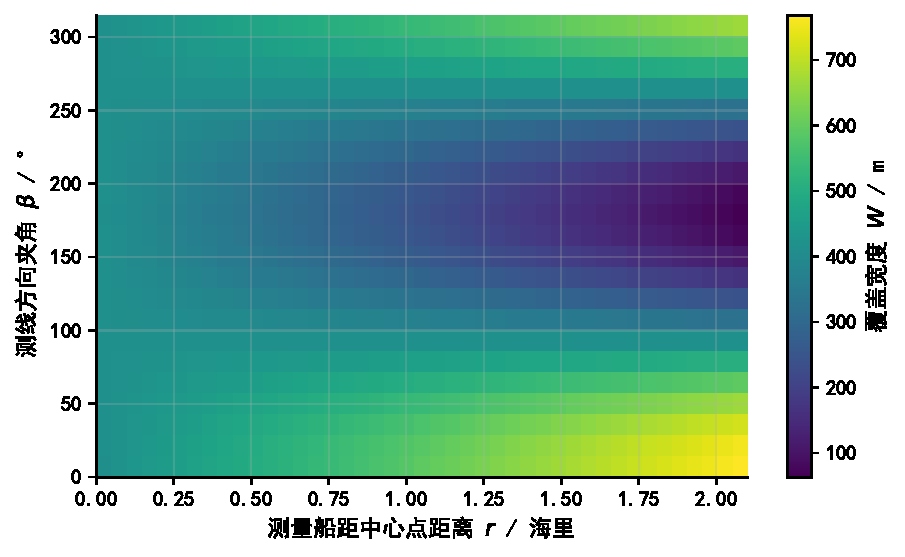
\includegraphics[width=0.78\textwidth]{../figures/q2/fig_q2_heatmap.pdf}
  \caption{覆盖宽度随测线方向夹角与船位距离的变化}
  \label{fig:q2_heatmap}
\end{figure}

\subsection{模型验证与本问结论}

当 $\beta=0^\circ$ 或 $180^\circ$ 时，测线方向沿坡面法向水平投影，垂直测线剖面沿等深线方向，$\alpha_{\mathrm{eff}}=0$，公式退化为平底公式 $W=2D\tan(\theta/2)$；当 $\beta=90^\circ$ 或 $270^\circ$ 时，船沿等深线运动，$D(r,\beta)=D_0$，覆盖宽度不随距离变化，与表 3 中该两行恒为 $416.55\text{ m}$ 一致。整体上覆盖宽度随水深增大而增大，$\beta=0^\circ$ 行随距离显著增大、$\beta=180^\circ$ 行随距离显著减小，符合物理直觉。
